% !TeX root = surprises.tex

\chapter{Ramsey Theory}\label{c.ramsey}

\abstract*{Ramsey theory is a branch of combinatorics that asks questions of the form: How large must a set be so that if it is divided into subsets, at least one subset has a certain property?
We present simple cases of four problems: Schur triples, Pythagorean triples, van der Waarden's problem and Ramsey's theorem. An overview is given of SAT solving, the method used to solve the Pythagorean triples problem.}

%%%%%%%%%%%%%%%%%%%%%%%%%%%%%%%%%%%%%%%%%%%%%%%%%%%%%%%%%%%

Ramsey theory is a branch of combinatorics that asks questions of the form: How large must a set be so that if it is divided into subsets, at least one subset has a certain property?
Results in Ramsey theory are difficult to prove and there remain many open problems. In this chapter we present simple cases of four problems to give a flavor of this fascinating subject: Schur triples (Sect.~\ref{s.schur}), triples of integers such that $a+b=c$, Pythagorean triples (Sect.~\ref{s.pyth}), triples of integers such that $a^2+b^2=c^2$, van der Waarden's problem (Sect.~\ref{s.van}) which concerns sequences of numbers, and Ramsey's theorem (Sect.~\ref{s.ramsey}) on coloring graphs.

Section~\ref{s.bounds} gives a taste of the probabilistic method in combinatorics by using the method to develop a lower bound for Ramsey numbers.

The Pythagorean triples problem was recently solved with the aid of computers, using a relatively new method call SAT solving. For readers familiar with propositional logic, Sect.~\ref{s.sat} gives an overview of how this is done.

Section~\ref{s.plimpton} describes Pythagorean triples as known to the Babylonians four thousand years ago.

Terminology: \emph{monochromatic} means \emph{of the same color}.

%%%%%%%%%%%%%%%%%%%%%%%%%%%%%%%%%%%%%%%%%%%%%%%%%%%%%%%%%%%
\vspace{-3ex}

\section{Schur triples}\label{s.schur}
\index{Schur triples}

\begin{definition}
Given \emph{any} decomposition of the set of positive integers \[S(n)=\{1,\ldots,n\}\]
into two disjoint subsets $S_1,S_2$, do there exist $a,b,c\in S_i$, $a\!<\!b\!<\!c$, such that $a+b=c$, for at least one $S_1,S_2$? If so, the set $\{a,b,c\}$ is called a \emph{Schur triple}.
\end{definition}

\begin{example} For $n=8$, in the decomposition:
\begin{align}
S_1 = \{1,2,3,4\},\; S_2 = \{5,6,7,8\}\,,
\label{eq.schur0}
\end{align}
the set $S_1$ includes the Schur triple $\{1,2,3\}$.
However, the decomposition:
\begin{align}
S'_1 = \{1,2,4,8\},\; S'_2 = \{3,5,6,7\}\,,
\label{eq:schur1}
\end{align}
does not contain a Schur triple, as you can check by enumerating all the triples in each subset.
\end{example}

\begin{theorem}
In \emph{all} decompositions of $S(9)=\{1,\ldots,9\}$ into two disjoint subsets, at least one subset contains a Schur triple.
\end{theorem}
Of course we could check the $2^9=512$ decompositions of $S(9)$ into two disjoint subsets, but let us try come up with a more succinct proof.
\begin{proof}
We try to construct a decomposition that \emph{does not} contain a Schur triple and show that the constraints of the problem make this impossible. Start by placing $1$ and $3$ into the subset $S_1$. $2$ must be placed in $S_2$ because $1+2=3$ and we are trying to construct a decomposition that does not contain a Schur triple. Similarly, $4$ must be placed in $S_2$ because $1+3=4$. Continuing, $6$ is placed in $S_1$ because $2+4=6$ and $7$ is placed in $S_2$ because $1+6=7$. However, $3+6=9$ and $2+7=9$, so $9$ must appear in both $S_1$ and $S_2$, a contradiction. The sequence of inferences is shown in the following table:
\[
\begin{array}{l@{\hspace{2em}}l}
S_1&S_2\\\svhline
1,3 & \\
1,3 & 2\\
1,3 & 2,4\\
1,3,6 & 2,4\\
1,3,6 & 2,4,7\\
1,3,6,9 & 2,4,7\\
1,3,6,9 & 2,4,7,9
\end{array}
\]
Backtracking, we search for a decomposition where $1,3$ are in different subsets. If we place $5$ into $S_2$, a sequence of inferences again leads to a contradiction because $9$ must appear in both subsets. The reader should justify each of the inferences shown in the following table:
\[
\begin{array}{l@{\hspace{2em}}l}
S_1&S_2\\\svhline
1&3\\
1 & 3,5\\
1,2&3,5\\
1,2,8&3,5\\
1,2,8&3,5,7\\
1,2,8&3,5,7,9\\
1,2,8&3,5,6,7,9\\
1,2,8,9&3,5,6,7,9
\end{array}
\]

\newpage

Backtracking again, we try to place $5$ into $S_1$, but that also leads to a contradiction, as shown in the following table:
\[
\begin{array}{l@{\hspace{2em}}l}
S_1&S_2\\\svhline
1&3\\
1,5& 3\\
1,5&3,4\\
1,5&3,4,6\\
1,2,5&3,4,6\\
1,2,5&3,4,6,7\\
1,2,5,7&3,4,6,7
\end{array}
\]

If follows that there is no decomposition that does not include a Schur triple.
\end{proof}

The theorem by Issai Schur\index{Schur, Issai} generalizes this example to dividing a set into $k$ subsets. For every $k$ there is a smallest $n$ such that in any decomposition of $S(n)$ into $k$ subsets, one of the subsets must contain a Schur triple.

%%%%%%%%%%%%%%%%%%%%%%%%%%%%%%%%%%%%%%%%%%%%%%%%%%%%%%%%%%%

\section{Pythagorean Triples}\label{s.pyth}

\begin{definition}
Given \emph{any} decomposition of the set of positive integers
\[S(n)=\{1,\ldots,n\}\]
into two disjoint subsets $S_1,S_2$, do there exist $a,b,c\in S_i$, $a\!<\!b\!<\!c$, such that $a^2+b^2=c^2$, for at least one of $S_1,S_2$? If so, $\{a,b,c\}$ is called a \emph{Pythagorean triple}.\index{Pythagorean triples}
\end{definition}

\begin{example}
For $n=10$, in the decomposition into even and odd numbers:
\[
S_1 = \{1,3,5,7,9\},\; S_2=\{2,4,6,8,10\}\,,
\]
there are no Pythagorean triples in $S_1$ but $\{6,8,10\}$ in $S_2$ is a Pythagorean triple since $6^2+8^2=10^2$.
\end{example}

Marijn J.H. Heule\index{Heule, Marijn J.H.} and Oliver Kullmann\index{Kullman, Oliver} proved the following theorems. Their method of proof is discussed in Sect.~\ref{s.sat}.

\begin{theorem}
For all $n\leq 7824$, there is \emph{some} decomposition of $S(n)$ into two disjoint subsets, such that both subsets \emph{do not contain} a Pythagorean triple.
\end{theorem}

\begin{theorem}
For all $n\geq 7825$, in \emph{all} decompositions of $S(n)$ into two disjoint subsets, at least one subset \emph{contains} a Pythagorean triple.
\end{theorem}
It is impossible to check all $2^{7825}$ decompositions of $S(7825)$. If we could check one decomposition every microsecond, $2^{7825}$ microseconds is approximately $10^{600}$ years, while the estimated age of the universe is only about $10^{10}$ years.



%%%%%%%%%%%%%%%%%%%%%%%%%%%%%%%%%%%%%%%%%%%%%%%%%%%%%%%%%%%

\section{Van der Waerden's problem}\label{s.van}

Consider the sequences of colored dots in Fig.~\ref{f.vdw1}. In the top sequence there are red dots at positions $(1,2,3)$ and blue dots at positions $(4,5,6)$. In each case, the positions form an arithmetic progression. Similarly, in the middle sequence the red dots at positions $(1,3,5)$ form an arithmetic progression. However, in the bottom sequence there is no set of three monochromatic dots whose positions form an arithmetic progression. 
Triples of red dots are at positions $(1,2,5)$, $(1,2,6)$, $(2,5,6)$, none of which form arithmetic progressions, and similarly for the blue dots.

\begin{figure}[htb]
\begin{center}
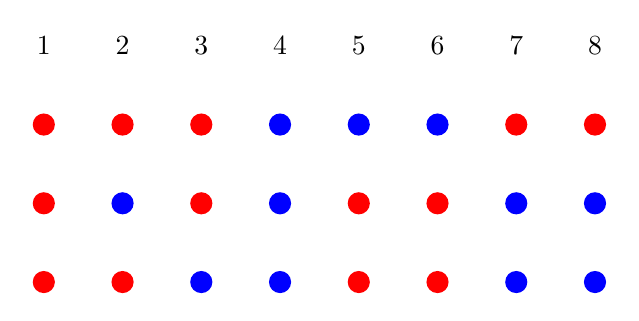
\begin{tikzpicture}
\foreach \x in {1,2,3,4,5,6,7,8} {
  \node at (\x,3) {$\x$};
}
\foreach \x/\col in {1/red,2/red,3/red,4/blue,5/blue,6/blue,7/red,8/red} {
  \fill[\col] (\x,2) circle(4pt);
}
\foreach \x/\col in {1/red,2/blue,3/red,4/blue,5/red,6/red,7/blue,8/blue} {
  \fill[\col] (\x,1) circle(4pt);
}
\foreach \x/\col in {1/red,2/red,3/blue,4/blue,5/red,6/red,7/blue,8/blue} {
  \fill[\col] (\x,0) circle(4pt);
}
\end{tikzpicture}
\end{center}
\caption{van der Waerden's problem for eight colored dots}\label{f.vdw1}
\end{figure}

With nine dots any coloring must contain a sequence of three monochromatic dots that form an arithmetic progression. Let us add an additional dot at the end of the bottom sequence in Fig.~\ref{f.vdw1} to obtain the sequences in Fig.~\ref{f.vdw2}. In the top sequence there are red dots at positions $(1,5,9)$, an arithmetic progression, and in the bottom sequence there are blue dots at positions $(7,8,9)$, also an arithmetic progression.
\begin{figure}[htb]
\begin{center}
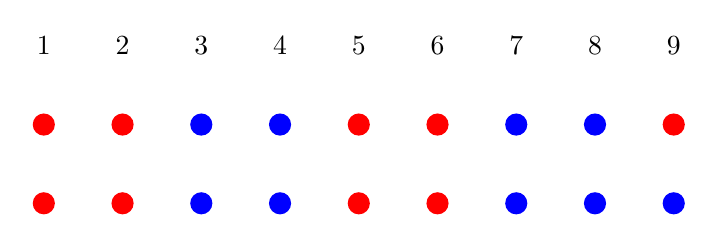
\begin{tikzpicture}
\foreach \x in {1,2,3,4,5,6,7,8,9} {
  \node at (\x,2) {$\x$};
}
\foreach \x/\col in {1/red,2/red,3/blue,4/blue,5/red,6/red,7/blue,8/blue,9/red} {
  \fill[\col] (\x,1) circle(4pt);
}
\foreach \x/\col in {1/red,2/red,3/blue,4/blue,5/red,6/red,7/blue,8/blue,9/blue} {
  \fill[\col] (\x,0) circle(4pt);
}
\end{tikzpicture}
\end{center}
\caption{van der Waerden's problem for nine colored dots}\label{f.vdw2}
\end{figure}


Bartel L. van der Waerden\index{van der Waerden, Bartel L.} posed the following\index{van der Waerden's problem} problem: For any positive integer $k$, what is the smallest number $n$ such that \emph{any} sequence of $n$ colored dots contains a sequence of $k$ monochromatic dots that form an arithmetic progression? For $k=3$, $n=9$, as demonstrated above for one decomposition. The next result is more difficult to show: for $k=4$, $n=35$.


%%%%%%%%%%%%%%%%%%%%%%%%%%%%%%%%%%%%%%%%%%%%%%%%%%%%%%%%%%%


\section{Ramsey's Theorem}\label{s.ramsey}

Color the edges of $K_5$, the complete graph on $5$ vertices, with two colors as shown in Fig.~\ref{f.ramsey5}. There are no monochromatic subgraphs $K_3$ (triangles) in the graph. Figure~\ref{f.ramsey6} shows one coloring of $K_6$ and it is easy to see that there are monochromatic triangles $\triangle ACE$ and $\triangle BDF$. In this section we prove a simple case of a theorem by Frank P. Ramsey\index{Ramsey, Frank P.} on the existence of subsets with a certain property.
\begin{figure}[ht]
\subfigures
\leftfigure[c]{
\begin{tikzpicture}
\node (pentagon) [minimum size=5cm,regular polygon,regular polygon sides=5] at (0,0) {};
\draw[red]  (pentagon.corner 1) node[black,above] {$A$} -- (pentagon.corner 2);
\draw[red]  (pentagon.corner 2) node[black,left] {$B$} -- (pentagon.corner 3);
\draw[red]  (pentagon.corner 3) node[black,left] {$C$} -- (pentagon.corner 4);
\draw[red]  (pentagon.corner 4) node[black,right] {$D$} -- (pentagon.corner 5);
\draw[red]  (pentagon.corner 5) node[black,right] {$E$} -- (pentagon.corner 1);
\draw[dashed,blue] (pentagon.corner 1) -- (pentagon.corner 3);
\draw[dashed,blue] (pentagon.corner 1) -- (pentagon.corner 4);
\draw[dashed,blue] (pentagon.corner 2) -- (pentagon.corner 4);
\draw[dashed,blue] (pentagon.corner 2) -- (pentagon.corner 5);
\draw[dashed,blue] (pentagon.corner 3) -- (pentagon.corner 5);
\end{tikzpicture}
}
\hfill
\rightfigure[c]{
\begin{tikzpicture}
\node (hexagon) [minimum size=5cm,regular polygon,regular polygon sides=6] at (0,0) {};
\draw[red]  (hexagon.corner 1) node[black,above] {$A$} -- (hexagon.corner 2);
\draw[red]  (hexagon.corner 2) node[black,above] {$B$} -- (hexagon.corner 3);
\draw[red]  (hexagon.corner 3) node[black,left] {$C$} -- (hexagon.corner 4);
\draw[red]  (hexagon.corner 4) node[black,left] {$D$} -- (hexagon.corner 5);
\draw[red]  (hexagon.corner 5) node[black,right] {$E$} -- (hexagon.corner 6);
\draw[red]  (hexagon.corner 6) node[black,right] {$F$} -- (hexagon.corner 1);
\draw[dashed,blue] (hexagon.corner 1) -- (hexagon.corner 3);
\draw[dashed,blue] (hexagon.corner 1) -- (hexagon.corner 4);
\draw[dashed,blue] (hexagon.corner 1) -- (hexagon.corner 5);
\draw[dashed,blue] (hexagon.corner 2) -- (hexagon.corner 4);
\draw[dashed,blue] (hexagon.corner 2) -- (hexagon.corner 5);
\draw[dashed,blue] (hexagon.corner 2) -- (hexagon.corner 6);
\draw[dashed,blue] (hexagon.corner 3) -- (hexagon.corner 5);
\draw[dashed,blue] (hexagon.corner 3) -- (hexagon.corner 6);
\draw[dashed,blue] (hexagon.corner 4) -- (hexagon.corner 6);
\end{tikzpicture}
}
\leftcaption{A coloring of $K_5$ with two colors}\label{f.ramsey5}
\rightcaption{A coloring $K_6$ with two colors}\label{f.ramsey6}
\end{figure}


\begin{definition}
$R(k)$, the \emph{Ramsey number} for $k$, is the smallest number $n$ such that in \emph{any} coloring of $K_{n}$, the complete graph on $n$ vertices, with two colors there is a monochromatic complete subgraph $K_k$.
\end{definition}
\index{Ramsey's theorem}
\begin{theorem}[Ramsey]
$R(3)=6$.\label{thm.ramsey}
\end{theorem}

\begin{proof}\index{Ramsey's theorem!proof that $R(3)=6$}
Figure~\ref{f.ramsey5} shows that $R(3)>5$. To show that $R(3)\leq 6$, consider any vertex $v$ in $K_6$. $v$ is connected to five other vertices, and when the edges are colored with two colors there must be at least three monochromatic edges incident with $v$. In Fig.~\ref{f.ramsey4a}, $\overline{AB}, \overline{AC}, \overline{AE}$ are colored red. Since the graph is complete all the vertices are connected, so if any one of the edges $\overline{BC}$, $\overline{BE}$, $\overline{CE}$ is colored red, say $\overline{BE}$, a red triangle $\triangle ABE$ is formed. Otherwise, all three edges of these edges are colored blue and they form a blue triangle (Fig.~\ref{f.ramsey4b}).
\end{proof}

The theorem can be generalized to any number of colors, as well as to colorings where the sizes of the subgraphs are not the same. $R(r,b,g)$ is the smallest complete graph such that  in any coloring with three colors there must be complete subgraphs with $r$ red edges, $b$ blue edges and $g$ green edges.

\begin{figure}[t]
\subfigures
\leftfigure[c]{
\begin{tikzpicture}
\node (hexagon) [minimum size=5cm,regular polygon,regular polygon sides=6] at (0,0) {};
\draw[red]  (hexagon.corner 1) node[black,above] {$A$} -- (hexagon.corner 2) node[black,above] {$B$};
\draw[blue,dashed]  (hexagon.corner 1) -- (hexagon.corner 6) node[black,right] {$F$};
\draw[red] (hexagon.corner 1) -- (hexagon.corner 3) node[black,below] {$C$};
\draw[blue,dashed] (hexagon.corner 1) -- (hexagon.corner 4) node[black,right] {$D$};
\draw[red] (hexagon.corner 1) -- (hexagon.corner 5) node[black,right] {$E$};
\end{tikzpicture}
}
\hfill
\rightfigure[c]{
\begin{tikzpicture}
\node (hexagon) [minimum size=5cm,regular polygon,regular polygon sides=6] at (0,0) {};
\draw[very thick,red]  (hexagon.corner 1) node[black,above] {$A$} -- (hexagon.corner 2) node[black,above] {$B$};
\draw[blue,dashed]  (hexagon.corner 1) -- (hexagon.corner 6) node[black,right] {$F$};
\draw[red] (hexagon.corner 1) -- (hexagon.corner 3) node[black,below] {$C$};
\draw[blue,dashed] (hexagon.corner 1) -- (hexagon.corner 4) node[black,right] {$D$};
\draw[very thick,red] (hexagon.corner 1) -- (hexagon.corner 5) node[black,right] {$E$};
\draw[very thick,red] (hexagon.corner 2) -- (hexagon.corner 5);
\draw[very thick,blue,dashed] (hexagon.corner 2) -- (hexagon.corner 3);
\draw[very thick,blue,dashed] ($(hexagon.corner 2)+(-2pt,0)$) -- ($(hexagon.corner 5)+(-2pt,0)$);
\draw[very thick,blue,dashed] (hexagon.corner 5) -- (hexagon.corner 3);
\end{tikzpicture}
}
\leftcaption{One vertex of $K_6$}\label{f.ramsey4a}
\rightcaption{Monochromatic triangles in $K_6$}\label{f.ramsey4b}
\end{figure}

%%%%%%%%%%%%%%%%%%%%%%%%%%%%%%%%%%%%%%%%%%%%%%%%%%%%%%%%%%%

\section{The Probabilistic Method}\label{s.bounds}

The only known non-trivial Ramsey numbers are $R(3)=6$ and $R(4)=18$. In 1947 Paul Erd\H{o}s\index{Paul Erdos@Paul Erd\H{o}s} developed the \emph{probabilistic method}\index{Probabilistic method} and used it to show lower and upper bounds on $R(k)$.\index{Ramsey's theorem!lower bound} Subsequent research has improved both bounds, but this is still a significant research area since the bounds are not tight. For example, it has been proved that $43\leq R(5) \leq 48$ and $798\leq R(10)\leq 23556$. In this section elementary probability is used to obtain a lower bound on $R(k)$.

To show that there exists an element of a set $S$ that has property $A$, prove that the probability of a \emph{random} element of $S$ having property $A$ is greater than zero. It is important to understand that the method is \emph{non-constructive}: it just proves that such an element exists but does not construct one. Although from Thm.~\ref{thm.ramsey} we know that $R(3)=6$, let us use the probabilistic method to obtain a lower bound for $R(3)$.\index{Ramsey's theorem!lower bound for}

\begin{theorem}[Erd\H{o}s]
$R(3) > 4$.
\end{theorem}
\begin{proof}
Given a \emph{random} coloring of $K_n$ by the two colors red and blue, consider an arbitrary subgraph $K_3$, that is, an arbitrary triangle with $\binom{3}{2}=3$ sides. The probability that all sides are colored red is $2^{-3}$, as is the probability that all sides are colored blue. Therefore, the probability that the triangle is monochromatic is $2\cdot 2^{-3}=2^{-2}=1/4$. The number of triangles in $K_n$ is $\binom{n}{3}$, so $P(n,3)$, the probability that $\emph{some}$ triangle contained in a random coloring of $K_n$ is monochromatic, is:
\[
P(n,3)=\binom{n}{3}\cdot \frac{1}{4}\,.
\]
If $P(n,3)<1$ then its complement $\overline{P}(n,3)=1-P>0$, that is, the probability that a random coloring of $K_n$ does \emph{not} contain a monochromatic triangle is greater than zero, so at least one must exist.

The following table shows $\overline{P}(n,3)$ for several values of $n$, and whether the value of $\overline{P}(n,3)$ proves that there exists a coloring with no monochromatic triangle:
\[
\renewcommand*{\arraystretch}{1.1}
\begin{array}{r@{\hspace{5mm}}r@{\hspace{5mm}}r}
\hline
\noalign{\smallskip}
n & \overline{P}(n,3) & \textit{Exists}\\
\noalign{\smallskip}\svhline\noalign{\smallskip}
3 & 3/4 & \textit{yes} \\
4 & 5/6 & \textit{yes}\\
5 & -3/7 & \textrm{--}\\
\noalign{\smallskip}
 \hline
 \end{array}
\]
\end{proof}
At first glance the result is strange because Fig.~\ref{f.ramsey5} shows that there exists a coloring of $K_5$ with no monochromatic coloring. However, the probabilistic criterion is sufficient but not necessary; it is a lower bound, meaning that $R(n)>4$ which is true because Thm.~\ref{thm.ramsey} showed that $R(n)=6$.

The same proof works for arbitrary $k$, so the probability of the existence of a coloring of $K_n$ with no monochromatic complete graph $K_k$ is:
\[
P(n,k)=\binom{n}{k}\cdot 2\cdot 2^{-\binom{k}{2}}\,.
\]
For $k=4$:
\begin{eqnarray*}
\overline{P}(n,4)&=&1-\binom{n}{4}\cdot 2^{-5}=\left(32-\binom{n}{4}\right)/32\\
\overline{P}(6,4)&=&(32-15)/32=17/32\\
\overline{P}(7,4)&=&(32-35)/32=-3/32\,.
\end{eqnarray*}
If follows that $R(4)>6$ which is much less than the known value $R(4)=18$.


%%%%%%%%%%%%%%%%%%%%%%%%%%%%%%%%%%%%%%%%%%%%%%%%%%%%%%%%%%%

\section{SAT Solving}\label{s.sat}

SAT solving is a method for solving problems that works by encoding a problem as a formula in propositional logic and then using a computer program to check the truth value of the formula. Advances in algorithms and implementations have made SAT solving a viable approach for problem solving. We give an overview of SAT solving and explain how it can be used to solve the mathematical problems described in this chapter. An elementary knowledge of propositional logic is assumed.\index{Propositional logic}

\subsection{Propositional Logic and the SAT Problem}

\begin{definition}\mbox{}\\
\vspace{-2ex}
\begin{itemize}
\item A \emph{formula} is composed of \emph{atomic formulas} or \emph{atoms} connected by the propositional operators $\vee$ (disjunction, ``or''), $\wedge$ (conjunction, ``and''), $\neg$ (negation, ``not'').
\item A formula is given an \emph{interpretation} by an assignment of $T$ or $F$ to each atom. Evaluating a formula in an interpretation results in its \emph{truth value} $T$ or $F$. (The reader is assumed to know how to evaluate a formula.)
\item A formula is \emph{satisfiable} if and only if there is an interpretation that makes its truth value $T$. Otherwise, the formula is \emph{unsatisfiable}.
\item A formula is in \emph{conjunctive normal form (CNF)} if and only if it is composed of a conjunction of subformulas each of which is a disjunction of \emph{literals} (atoms or negations of atoms).
\end{itemize}
\end{definition}

The following formula is in CNF:
\[
(\neg p \vee q \vee \neg \,r) \;\wedge\; (\neg p \vee r)
\;\wedge\; (\neg \,r)\;\wedge\;(p \vee q \vee \neg \,r)\,.
\]

The \emph{SAT problem} is to decide if a given formula in CNF is satisfiable or not. A \emph{SAT solver}\index{SAT solver} is a computer program that can solve the SAT problem. Most SAT solvers are based on the DPLL algorithm which goes back to the 1960's, but recent developments have made very significant improvements to the algorithm. Highly optimized implementations of these algorithms have made SAT solvers an important tool for solving problems in many fields including mathematics.

\newpage

\section{Solving Schur triples}\index{Schur triples}

Let us encode the Schur triples problem $S(8)$ as a formula in CNF. The formula will be satisfiable if and only if there is a decomposition of a set $S$, so that neither $S_1$ nor $S_2$ contains a Schur triple. There is an atom $p_i$ for each of the numbers $1\leq i \leq 8$. The intended meaning of an interpretation for the formula is that it assigns $T$ to $p_i$ if $i$ is in the first subset $S_1$ and $F$ if $i$ is in the second subset $S_2$. To show that in all decompositions neither subset contains a Schur triple, the interpretation must ensure that for each possible Schur triple at least one atom is assigned $T$ and one atom is assigned $F$. 

For example, $(2,4,6)$ is a Schur triple, so at least one of the three integers must be in $S_1$ and at least one of them must be in $S_2$. Therefore, $p_2 \vee p_4 \vee p_6$ must be true and also $\neg p_2 \vee \neg p_4 \vee \neg p_6$ must be true. There are $12$ possible Schur triples, so the CNF formula is:
\begin{align}
\begin{array}{l}
(p_1 \vee p_2 \vee p_3) \;\wedge\; (\neg p_1 \vee \neg p_2 \vee \neg p_3) \;\wedge \\
(p_1 \vee p_3 \vee p_4) \;\wedge\; (\neg p_1 \vee \neg p_3 \vee \neg p_4) \;\wedge \\
(p_1 \vee p_4 \vee p_5) \;\wedge\; (\neg p_1 \vee \neg p_4 \vee \neg p_5) \;\wedge \\
(p_1 \vee p_5 \vee p_6) \;\wedge\; (\neg p_1 \vee \neg p_5 \vee \neg p_6) \;\wedge \\
(p_1 \vee p_6 \vee p_7) \;\wedge\; (\neg p_1 \vee \neg p_6 \vee \neg p_7) \;\wedge \\
(p_1 \vee p_7 \vee p_8) \;\wedge\; (\neg p_1 \vee \neg p_7 \vee \neg p_8) \;\wedge \\
(p_2 \vee p_3 \vee p_5) \;\wedge\; (\neg p_2 \vee \neg p_3 \vee \neg p_5) \;\wedge \\
(p_2 \vee p_4 \vee p_6) \;\wedge\; (\neg p_2 \vee \neg p_4 \vee \neg p_6) \;\wedge \\
(p_2 \vee p_5 \vee p_7) \;\wedge\; (\neg p_2 \vee \neg p_5 \vee \neg p_7) \;\wedge \\
(p_2 \vee p_6 \vee p_8) \;\wedge\; (\neg p_2 \vee \neg p_6 \vee \neg p_8) \;\wedge \\
(p_3 \vee p_4 \vee p_7) \;\wedge\; (\neg p_3 \vee \neg p_4 \vee \neg p_7) \;\wedge \\
(p_3 \vee p_5 \vee p_8) \;\wedge\; (\neg p_3 \vee \neg p_5 \vee \neg p_8)\,.
\end{array}\label{eq.schur2}
\end{align}
When a SAT solver is given this formula, it answers that the formula is satisfiable under either of the interpretations:
\[
\begin{array}{c@{\hspace{8pt}}c@{\hspace{8pt}}c@{\hspace{8pt}}c@{\hspace{8pt}}c@{\hspace{8pt}}c@{\hspace{8pt}}c@{\hspace{8pt}}c}
p_1&p_2&p_3&p_4&p_5&p_6&p_7&p_8\\\svhline
F&F&T&F&T&T&T&F\\
T&T&F&T&F&F&F&T
\end{array}
\]
One interpretation corresponds to the decomposition in Eq.~\ref{eq:schur1}: 
$S_1=\{1,2,4,8\}$, $S_2=\{3,5,6,7\}$ while the other corresponds to the symmetrical decomposition $S_1=\{3,5,6,7\}$, $S_2=\{1,2,4,8\}$.

\newpage

For $S(9)$ four pairs of subformulas must be added for the additional possible Schur triples:
\[
\begin{array}{l}
(p_1 \vee p_8 \vee p_9) \;\wedge\; (\neg p_1 \vee \neg p_8 \vee \neg p_9) \;\wedge \\
(p_2 \vee p_7 \vee p_9) \;\wedge\; (\neg p_2 \vee \neg p_7 \vee \neg p_9) \;\wedge \\
(p_3 \vee p_6 \vee p_9) \;\wedge\; (\neg p_3 \vee \neg p_6 \vee \neg p_9) \;\wedge \\
(p_4 \vee p_5 \vee p_9) \;\wedge\; (\neg p_4 \vee \neg p_5 \vee \neg p_9)\,.
\end{array}
\]
When the SAT solver is given this formula, it answers that the formula is unsatisfiable, meaning that \emph{no} decomposition has \emph{no} Schur triple. Removing the double negative, this states that in \emph{every} decomposition of $S(9)$ there exists a Schur triple.

\subsection{Solving Pythagorean Triples}\index{Pythagorean triples}

Heule\index{Heule, Marijn J.J.} and Kullmann\index{Kullman, Oliver} solved the Pythagorean triple problem using a highly optimized SAT solver. There was a significant difference in efficiency between finding a decomposition that does not have Pythagorean triples (you just need one decomposition), and showing all that decompositions have a Pythagorean triple (you have to check all of them). To show that for all $S(n)$, $1\leq n\leq 7824$, there is a decomposition with no triple took only one minute of computing time, whereas to show that every decomposition of $S(7825)$ has a triple took about two days of computing time for a computer with $800$ \emph{cores} (processors) working in parallel, altogether $40,000$ hours of computing time!

The use of computers in mathematics naturally raises the question: Can we trust a proof generated by a computer? Of course, even ``ordinary'' mathematical proofs can be incorrect (see Sect.~\ref{s.kempe}), but our experience with frequent computer bugs, as well as the opaqueness of large computer programs, makes us more sensitive to potential errors in computer-generated proofs.

One approach to increasing confidence in the correctness of a computer-generated proof is to use two or more programs, written independently by two or more researchers. If the multiple programs are written in different programming languages and for different computers and operating systems, this lessens the possibility of a bug in the computer hardware and software.

Heule and Kullmann's SAT solver wrote out a log of the steps in the proof so that it could be examined for correctness. The log was so massive, $200$ terabytes, that it was impossible to examine directly. To put this into perspective, $200$ terabytes is $200,\!000$ gigabytes while your computer might have an internal memory of $16$ gigabytes and a solid-state disk of $128$ gigabytes. Instead, they wrote a small program to verify the correctness of the data in the log. To ensure that this program was correct, they wrote a formal proof using the Coq proof assistant that supports and checks the work of mathematicians without totally automating the proof process.

\subsection{An Overview of the DPLL Algorithm}\index{SAT solver!DPLL algorithm}

The first algorithm that one learns for SAT solving is \emph{truth tables}. Given a formula $A$ in propositional logic with $n$ different atoms, there are $2^n$ interpretations since each atom can be independently assigned $T$ or $F$. For each interpretation, it is straightforward to compute the truth value of $A$ using the definition of the propositional operators. However, to check $2^n$ interpretations is very inefficient for even moderately large $n$.

The DPLL algorithm works by incrementally assigning $T$ or $F$ to an atom and then attempting to evaluate the formula. For example, given $A=p \wedge q \wedge \neg\, r$, if $p$ is assigned $F$, then $A$ evaluates to $F$, regardless of the assignments to $q$ and $r$, and there is no need to perform further evaluations. Similarly, $A=p\vee q \vee \neg\, r$ evaluates to $T$ if $p$ is assigned $T$, regardless of the assignments to $q$ and $r$.

The efficiency of DPLL comes from \emph{unit propagation}.\index{SAT solver!unit propagation} Consider part of the formula for Schur triples:
\begin{align}
\begin{array}{l}\label{eq.schur3}
(p_1 \vee p_2 \vee p_3) \wedge (\neg p_1 \vee \neg p_2 \vee \neg p_3) \:\wedge \\
(p_1 \vee p_3 \vee p_4) \wedge (\neg p_1 \vee \neg p_3 \vee \neg p_4) \:\wedge \\
\cdots\\
(p_3 \vee p_4 \vee p_7) \wedge (\neg p_3 \vee \neg p_4 \vee \neg p_7) \:\wedge \\
(p_3 \vee p_5 \vee p_8) \wedge (\neg p_3 \vee \neg p_5 \vee \neg p_8)\,.
\end{array}
\end{align}
Suppose that we have assigned $F$ to $p_1,p_2$. The first subformula reduces to the unit formula consisting of the single atom $p_3$. If the formula is to be satisfiable, we \emph{must} assign $T$ to $p_3$ and all the subformulas:
\[
(p_1 \vee p_2 \vee p_3),\;(p_1 \vee p_3 \vee p_4),\;
(p_3 \vee p_4 \vee p_7),\;(p_3 \vee p_5 \vee p_8)\,,
\]
immediately evaluate to $T$.

Since $\neg p_3$ evaluates to $F$, each subformula can be satisfiable only if some other atom in a subformula containing $\neg p_3$ is assigned $T$. In $\neg p_3 \vee \neg p_5 \vee \neg p_8$, either $p_5$ or $p_8$ must be assigned $F$ so that either $\neg p_5$ or $\neg p_8$ evaluates to $T$.

The result of this analysis shows that once $p_1,p_2$ have been assigned $F$, the formula in Eq.~\ref{eq.schur3} is satisfiable if and only if $(\neg p_4 \vee \neg p_7) \:\wedge\: (\neg p_5 \vee \neg p_8)$ is satisfiable.

By performing the propagation of $p_3$ on all the subformulas of Eq.~\ref{eq.schur2}, the formula is reduced to:
\[
\begin{array}{l}
(p_4\vee p_5)\;\wedge\;(p_4\vee p_6)\;\wedge\;(p_5\vee p_6)\;\wedge\;(p_5\vee p_7)\;\wedge\;\\
(p_6\vee p_7)\;\wedge\;(p_6\vee p_8)\;\wedge\;(p_7\vee p_8)\;\wedge\\
(\neg p_4\vee \neg p_7)\;\wedge\;
(\neg p_5\vee \neg p_8)\,.
\end{array}
\]
One more assignment of $F$ to $p_4$ results in a satisfying interpretation which we have found after only three arbitrary assignments.

Advanced algorithms for SAT are based on using information that can be obtained from the current partially-evaluated formula to limit the number of arbitrary assignments that must be made.

%%%%%%%%%%%%%%%%%%%%%%%%%%%%%%%%%%%%%%%%%%%%%%%%%%%%%%%%%%%

\section{Pythagorean Triples in Babylonian Mathematics}\label{s.plimpton}

This section is a digression from Ramsey theory; it is included to give a taste of the rich theory of Pythagorean triples and to demonstrate the depth of mathematical knowledge in the ancient world. Pythagorean triples\index{Pythagorean triples} were known in Babylonian mathematics\index{Babylonian mathematics} since at least 1800 BCE.
\begin{definition}
A \emph{primitive Pythagorean triple}\index{Pythagorean triples!primitive} is a set of three positive integers $\{a,b,c\}$ such that $a^2+b^2=c^2$, and $a,b,c$ have no common factor greater than $1$.
\end{definition}
\begin{example}
$\{3,4,5\}$ is a primitive Pythagorean triple. $\{6,8,10\}$ is Pythagorean triple that is not primitive since $2$ as a common factor.
\end{example}
A cuneiform tablet called \emph{Plimpton $322$}\index{Plimpton 322} is one of the earliest examples of Babylonian mathematics. It lists fifteen primitive Pythagorean triples by giving $a$ and $c$. Table~\ref{t.babylonian} displays several of these triples, together with the computed values of $b$ and other values that will be discussed below.

Historians of mathematics have proposed several explanations for how these triples were found. One explanation is that \emph{Euclid's formula}\index{Euclid's formula} was used to obtain the triples from a pair of generating numbers.
\begin{theorem}[Euclid]
$\{a,b,c\}$ is primitive Pythagorean triple if and only if there exist two positive integers $u,v$, called \emph{generating numbers}, such that:\label{thm.euclid-function}
\begin{enumerate}
\item $u>v$
\item they are not both odd
\item they have no common factor greater than $1$
\item the following relations hold between $\{a,b,c\}$ and $u,v$:
\[
a=u^2-v^2,\quad b=2uv,\quad c=u^2+v^2\,.
\]
\end{enumerate}
\end{theorem}

\begin{table}[t]
\caption{Babylonian triples from the Plimpton $322$ tablet}\label{t.babylonian}
\[
\begin{array}{r@{$\quad\quad$}r@{$\quad\quad$}r@{$\quad\quad$}r@{$\quad\quad$}r@{$\quad\quad$}r@{$\quad\quad$}r@{$\quad\quad$}r@{$\quad\quad$}r}
\hline
\noalign{\smallskip}
a&a_{\textit{factors}}&b&b_{\textit{factors}}&c&u&u_{\textit{factors}}&v&v_{\textit{factors}}\\
\noalign{\smallskip}\svhline\noalign{\smallskip}
119&7\cdot 17 &120&2^3 \cdot 3\cdot 5 & 169&12&2^2\cdot 3&5&5\\
4601 &43\cdot 107&4800&2^6 \cdot 3 \cdot 5^2& 6649&75&3\cdot 5^2&32&2^5\\
12709 &71\cdot 179&13500&2^2 \cdot 3^3 \cdot 5^3& 18541&125&5^3&54&2\cdot 3^3\\
65 &5\cdot 13&72&2^3 \cdot 3^2 & 97&9&3^2&4&2^2\\
\noalign{\smallskip}\hline
\end{array}
\]
\end{table}

\begin{proof}
By computation it follows immediately that if $\{a,b,c\}$ can be expressed as required in item $4$ they form a Pythagorean triple:
\begin{eqnarray*}
a^2+b^2&=&(u^2-v^2)^2 + (2uv)^2\\
&=& u^4-2(uv)^2+v^4+4(uv)^2\\
&=&u^4+2(uv)^2+v^4\\
&=&u^2+v^2=c^2\,.
\end{eqnarray*}
The proof of the other direction is more complicated and is omitted.
\end{proof}
If it is true that the Babylonians used Euclid's formula, the question remains: How did they discover the generating numbers $u,v$?

Table~\ref{t.babylonian} displays $a_{\textit{factors}}$ and $b_{\textit{factors}}$, the factorizations of $a$ and $b$, respectively, showing that they have no common factors. The reader is invited to check that the $c$ has no common factor with  $a,b$ so the triples are primitive. $u,v$  and $u_{\textit{factors}}, v_{\textit{factors}}$ are also displayed. Not only do they not have any common factors as required by Thm.~\ref{thm.euclid-function}, but the only factors greater than $1$ in $u$ and $v$ are powers of $2,3,5$.
\begin{definition}
A \emph{Babylonian triple} is a primitive Pythagorean triple such that the only prime factors of $u,v$ are $2,3,5$.
\end{definition}
The reason that the Babylonians restricted themselves to these factors is that they used the \emph{sexagesimal}\index{Sexagesimal number system} or base $60$ number system whose prime factors are $2,3$ and $5$: $60=2\cdot 2\cdot 3\cdot 5$.

For readers who are not familiar with non-decimal number systems,  here is a brief overview of the concept. The ``number'' $12345$ is a shorthand for the number:
\[
(1\times 10^4) + (2\times 10^3) + (3\times 10^2) + (4\times 10^1) + (5\times 10^0)\,.
\]
This number system is called the \emph{decimal} or base $10$ number system. There are ten digits $0,1,2,\ldots,8,9$ for the coefficients of the powers, and the powers are represented by the places of coefficients with increasing powers from right to left. 

The number could also be represented in the binary or base $2$ number system by:
\[
12345=8192 + 4096 + 32+16+8+1=
2^{13} + 2^{12} + 2^{5} + 2^{4} + 2^{3} + 2^0=11000000111001\,,
\]
where in $2^{13} + 2^{12} + 2^{5} + 2^{4} + 2^{3} + 2^0$, powers of $2$ whose coefficient is $0$ are omitted. The coefficients of the remaining powers are $1$ and can also be omitted. $11000000111001$ is the number in binary notation which uses two digits $0,1$ for the coefficients and the powers of two are indicated by the places of the coefficients.

Another popular number system is the \emph{hexadecimal} or base $16$ number system which is used in computing. For this number system we need $16$ ``digits'' and the convention is to use $0,1,2,\ldots,8,9,A,B,C,D,E,F$.

The base $60$ number system is not as unfamiliar as it may seem, because we represent time, geographical coordinates and angles in that system. We are comfortable carrying out computations such as ($1$ hour $40$ minutes) plus ($1$ hour $30$ minutes) equals ($3$ hours $10$ minutes).

Table~\ref{t.sexagesimal} shows the values of $a,c$ that appear in the tablet in base $60$ notation where $\langle d\rangle$ represents the $d$'th ``digit'' for $0\leq d<60$.
\begin{table}[ht]
\caption{Babylonian triples in base $60$}\label{t.sexagesimal}
\[
\begin{array}{r@{$\quad\quad$}r}
\hline
\noalign{\smallskip}
a&c\\
\noalign{\smallskip}\svhline\noalign{\smallskip}
\langle 1\rangle \langle 59 \rangle&\langle 2\rangle \langle 49 \rangle\\
\langle 1\rangle \langle 16 \rangle\langle 41\rangle&\langle 1\rangle \langle 50 \rangle\langle 49\rangle\\
\langle 3\rangle \langle 31 \rangle\langle 49\rangle&\langle 5\rangle \langle 09 \rangle\langle 01\rangle\\
\langle 1\rangle \langle 05 \rangle&\langle 1\rangle \langle 37 \rangle\\
\noalign{\smallskip}\hline
\end{array}
\]
\end{table}

 The reader can check that these values are the same as the decimal values given in Table~\ref{t.babylonian}, for example:
\[
\renewcommand{\arraystretch}{1.3}
\begin{array}{lclclcr}
(3\times 60^2) &+& (31\times 60^1) &\;+\;& (49\times 60^0) &=& 12709\\
(5\times 60^2) &\;+\;& (9\times 60^1) &\;+\;& (1\times 60^0) &=&18541\,.
\end{array}
\]

The Babylonians did not have $60$ distinct symbols for the digits. Instead, they used a hybrid system where the coefficients were represented with two symbols, one for ones and one for tens, and the places of the coefficients indicated the powers of $60$. Using  $\heartsuit$ for tens and $\diamondsuit$ for ones, the decimal number $(38\times 60)+(16\times 60^0)=2296$ would be represented as:
\[
\heartsuit\heartsuit\heartsuit \; \stackrel{\displaystyle\diamondsuit\diamondsuit\diamondsuit\diamondsuit}{\diamondsuit\diamondsuit\diamondsuit\diamondsuit}
\quad
\heartsuit \; \stackrel{\displaystyle\diamondsuit\diamondsuit}{\diamondsuit\diamondsuit\diamondsuit\diamondsuit}\,.
\]

%%%%%%%%%%%%%%%%%%%%%%%%%%%%%%%%%%%%%%%%%%%%%%%%%%%%%%%%%%%

\subsection*{What Is the Surprise?}

Frank P. Ramsey's theorem \index{Ramsey, Frank P.} appeared to be a minor result in combinatorics. Surprisingly, the theorem was the foundation of an entirely new and challenging field of mathematics with many open problems. The nature of Ramsey theory is also surprising: if a set is large enough there exist regularities in its subsets.

I was introduced to Ramsey theory by the article by Marijn J. H. Heule\index{Heule, Marijn J. H.} and Oliver Kullmann\index{Kullman, Oliver}  on Pythagorean triples whose proof bears some similarity to the proof of the four-color theorem: the use of massive computing resources that is only successful after theoretical advances. Hence the title of their article: \textit{The Science of Brute Force}.

Problems in combinatorics ask for specific numerical values, for example, $R(n)$ must be a specific positive integer. It is surprising that probabilistic methods have proved so fruitful in obtaining results in this field.

We tend to think that humans are smarter today then they used to be thousands of years ago. It can be a surprise to find out that four thousand years ago Babylonian mathematics was sufficiently advanced to discover that $(12709, 13500, 18541)$ is a Pythagorean triple.

\subsection*{Sources}

For an overview of Ramsey theory see \cite{burton}, while an advanced presentation can be found in \cite{rudiments}. The section on the probabilistic method is based on \cite[Example~4o]{ross} and \cite[Chapter~4]{burton}. A database of Ramsey numbers can be found in \cite{mckay}.

The method of proof of the theorem on Pythagorean triples is explained in detail in \cite{brute}. See \cite{mlcs} for an introduction to logic and to SAT solving. The archive of my SAT solver for education \cite{joss} contains formulas for Schur triples, Ramsey graphs and van der Waerden's problem. 

Section~\ref{s.plimpton} is based upon \cite{wiki:plimpton}, \cite{robson}. 
The sexagesimal number system is described in \cite{wiki:sexagesimal}.
